\documentclass[11pt]{article}
% \usepackage[utf8]{inputenc}
\usepackage{amsmath, amstext, amsfonts}
\usepackage[pdftex]{graphicx,color}



\begin{document}


\section{Complex phase distribution and seismic velocity structure of the
transition zone}

Here we give a overview of the model setup.


\subsection{Model domain}
A 2D cylindrical model domain with an opening angle of $90^{\deg}$ is used. 
\subsubsection{Velocity}
The set of non dimensional equations that have to be solved (TALA),
\begin{eqnarray}
 \nabla \cdot (\rho_{r}\bf u) = 0 \\
-\nabla P + \nabla \cdot \tau = T Ra \bf e_{z}
\end{eqnarray} 
\subsubsection{viscosity}
for the viscosity we use the relation 
$\eta(T, z) = \eta_{0} e^{(cz -b T )}$ with 
$b = ln(\delta \eta T ), c = ln(\delta \eta P )$
\subsubsection{boundary conditions}
The boundary conditions for the velocity are free slip impermeable for all boundaries.
\subsubsection{Temperature}
The set of non dimensional equations that have to be solved
\begin{eqnarray}
\rho c_{p} \frac{DT}{Dt} - \alpha \rho u T = \partial_{j} (k\partial_{j} T) + \tau_{ij}\partial_{j}u_{i}  + \rho H
\end{eqnarray}
with $\alpha \rho u T $ heating due to adiabatic compression, $\tau_{ij}\partial_{j}u_{i}$ viscous heating and $\rho H$ radiogenic heating. \\
The model is heated in the interior with $2\times 10^{-12} W/kg$ slightly lower than the chondritic value in agreement with the smaller surface/volume ratio of the 2D cylinder.
\subsubsection{boundary conditions}
For the energy equation we prescribe a constant temperature at the bottom and top with a contrast of 3500K
the other boundaries prescribe zero heatflux.
\subsection{Physical properties}
The physical properties $\rho$, cp and $\alpha$
appear as coefficients and are included in our model through a general interface based on
pressure temperature (P, T ) domain tabulation of the coefficient values in the relevant pressure and
temperature range for the Earth’s mantle.
\subsection{Lookup table}
we need to use a lookup table for the evaluation of these physical properties that depend on pressure and temperature since the number of evaluations of these properties is roughly 200 per element.
$N_{eval} = (Nstokes + Nenergy ) \times 2 = (Ne \times ng + 3 \times Ne \times 4 \times ng ) \times 2 = 26 \times Ne \times ng$
This amounts to $Neval = 5.8 \times 10^{6}$ table evaluations per integration time step for the finite element mesh size used in our model calculations where Ne = 32000
\subsection{Initial conditions}
Since we have a non nonlinear relation between for instance Temperature and cp we need to apply an iterative procedure to generate the correct initial conditions or temperature and density. \\
For this purpose we start from a rough estimation of an adiabat truncated by two thermal boundary layers at the top and the bottom of the domain and iterate towards an equilibrium condition.
\begin{figure}
\centering
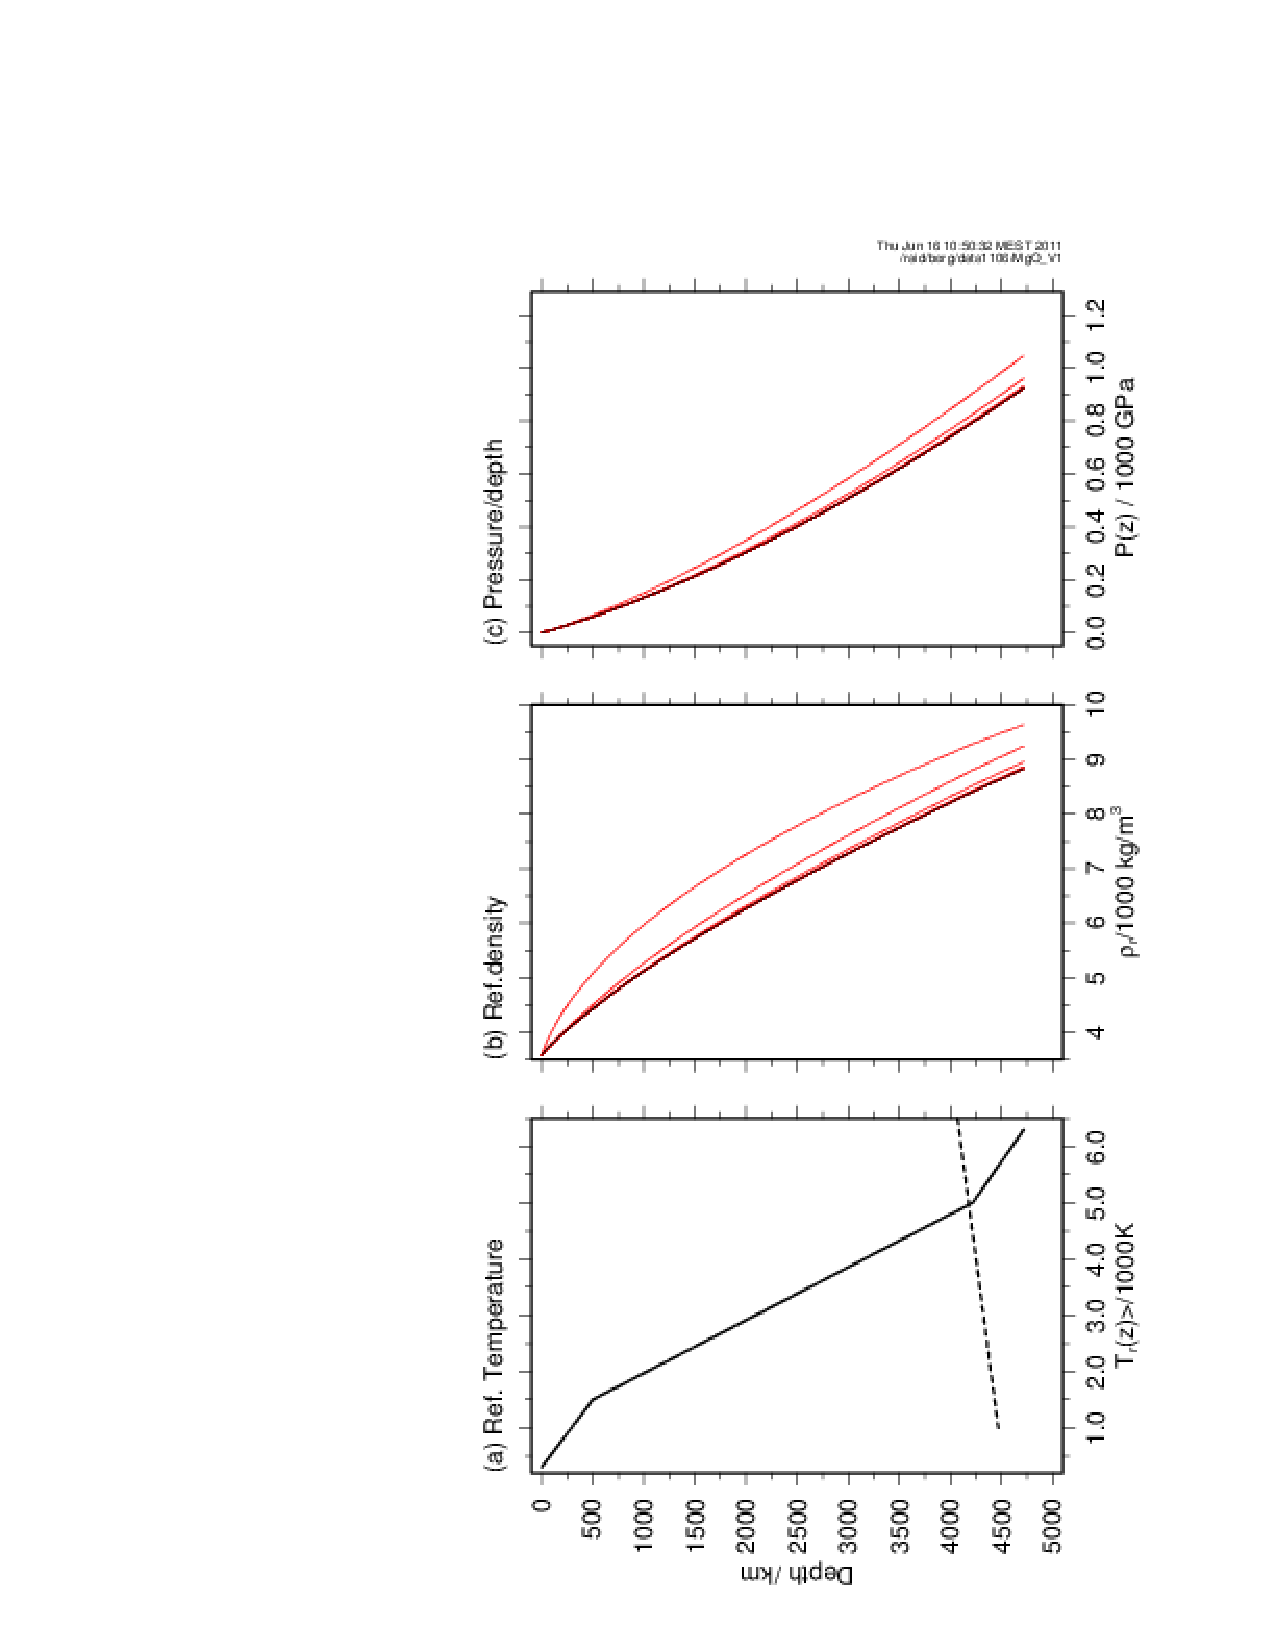
\includegraphics[width=\textwidth,angle=-90]{./profiles_refmod.pdf}
% profiles_refmod.pdf: 612x792 pixel, 72dpi, 21.59x27.94 cm, bb=0 0 612 792
\caption{the leftmost frame gives the initial geotherm. The frames on the right give the convergence towards an equilibrium state for density and pressure after several iterations. the black line gives the converged state}
\end{figure}

\end{document}
